\begin{figure}[p]
    \centering
    \begin{minipage}[b]{.48\textwidth}
        \begin{figure}[H]
            \centering
            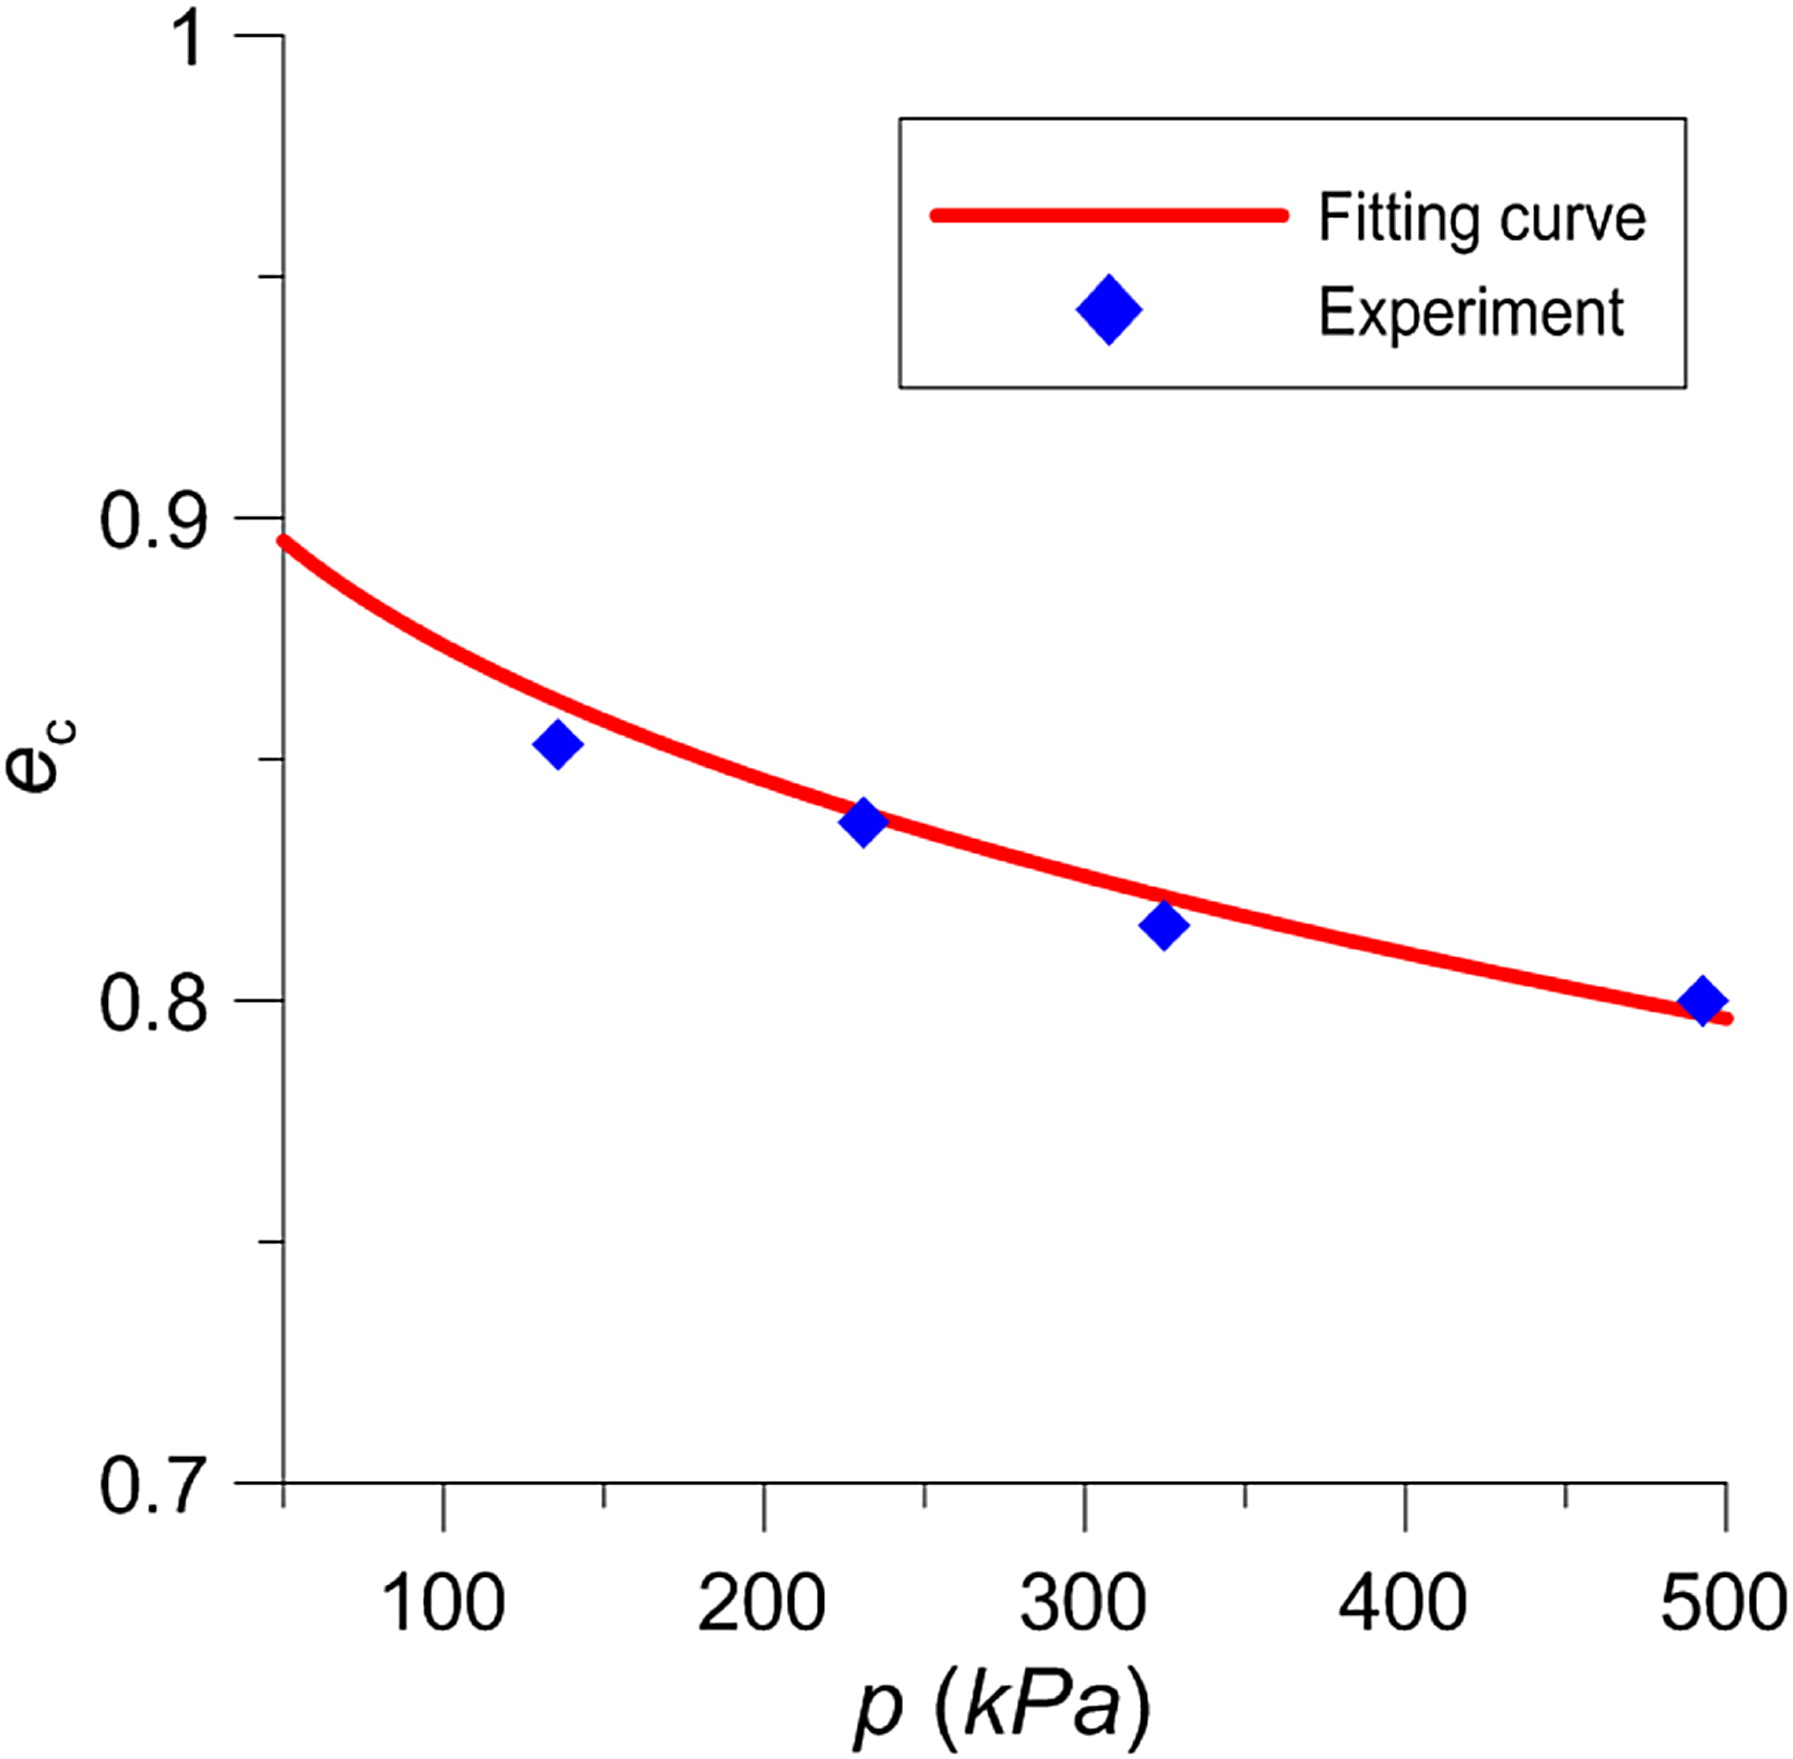
\includegraphics[width=.8\textwidth]{figures/figure8.jpg}
            \bicaption{The $e_c-p$ curve at critical state (experimental data from \citet{Chu2003})}{临界状态下的$e_c-p$曲线(实验数据来自\citealt{Chu2003})}
            \label{figure:8}
        \end{figure}
        \begin{figure}[H]
            \centering
            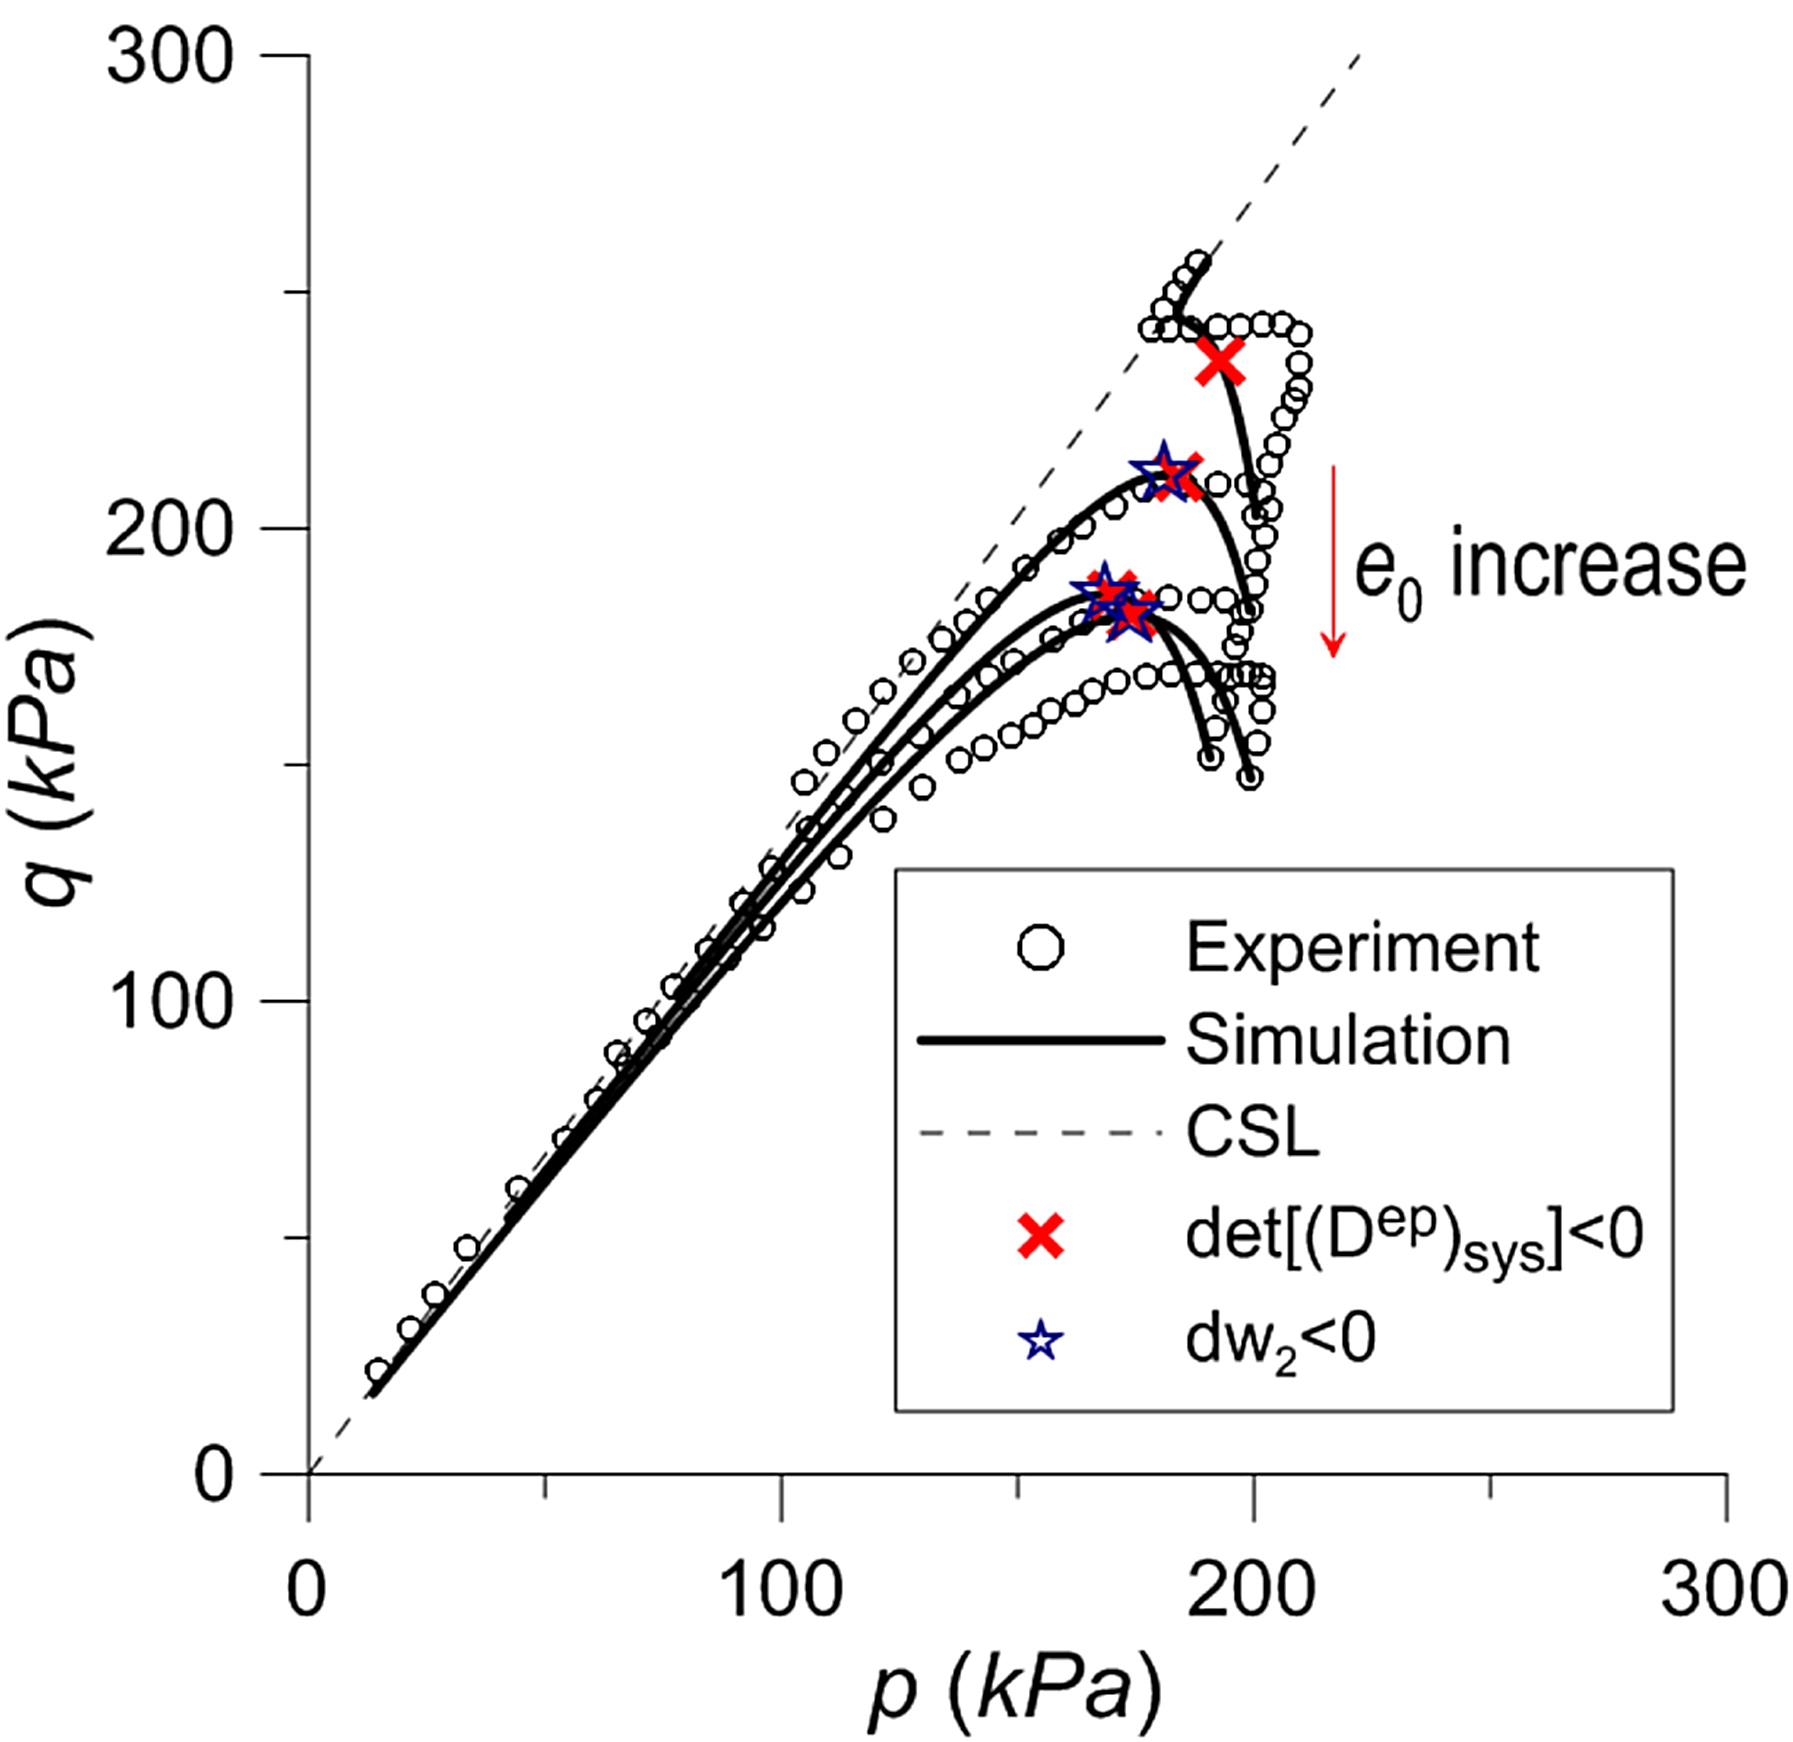
\includegraphics[width=.8\textwidth]{figures/figure9.jpg}
            \bicaption{Stress path of  $K_0$-consolidated undrained triaxial test (experimental data from \citealt{Chu2008})}{$K_0$固结三轴不排水试验的应力路径(实验数据来自\citealt{Chu2008})}
            \label{figure:9}
        \end{figure}
    \end{minipage}
    \hspace{0.02\textwidth}
    \begin{minipage}[b]{.48\textwidth}
        \begin{figure}[H]
            \centering
            \subfigure[stress-strain relationship 应力应变关系]{
                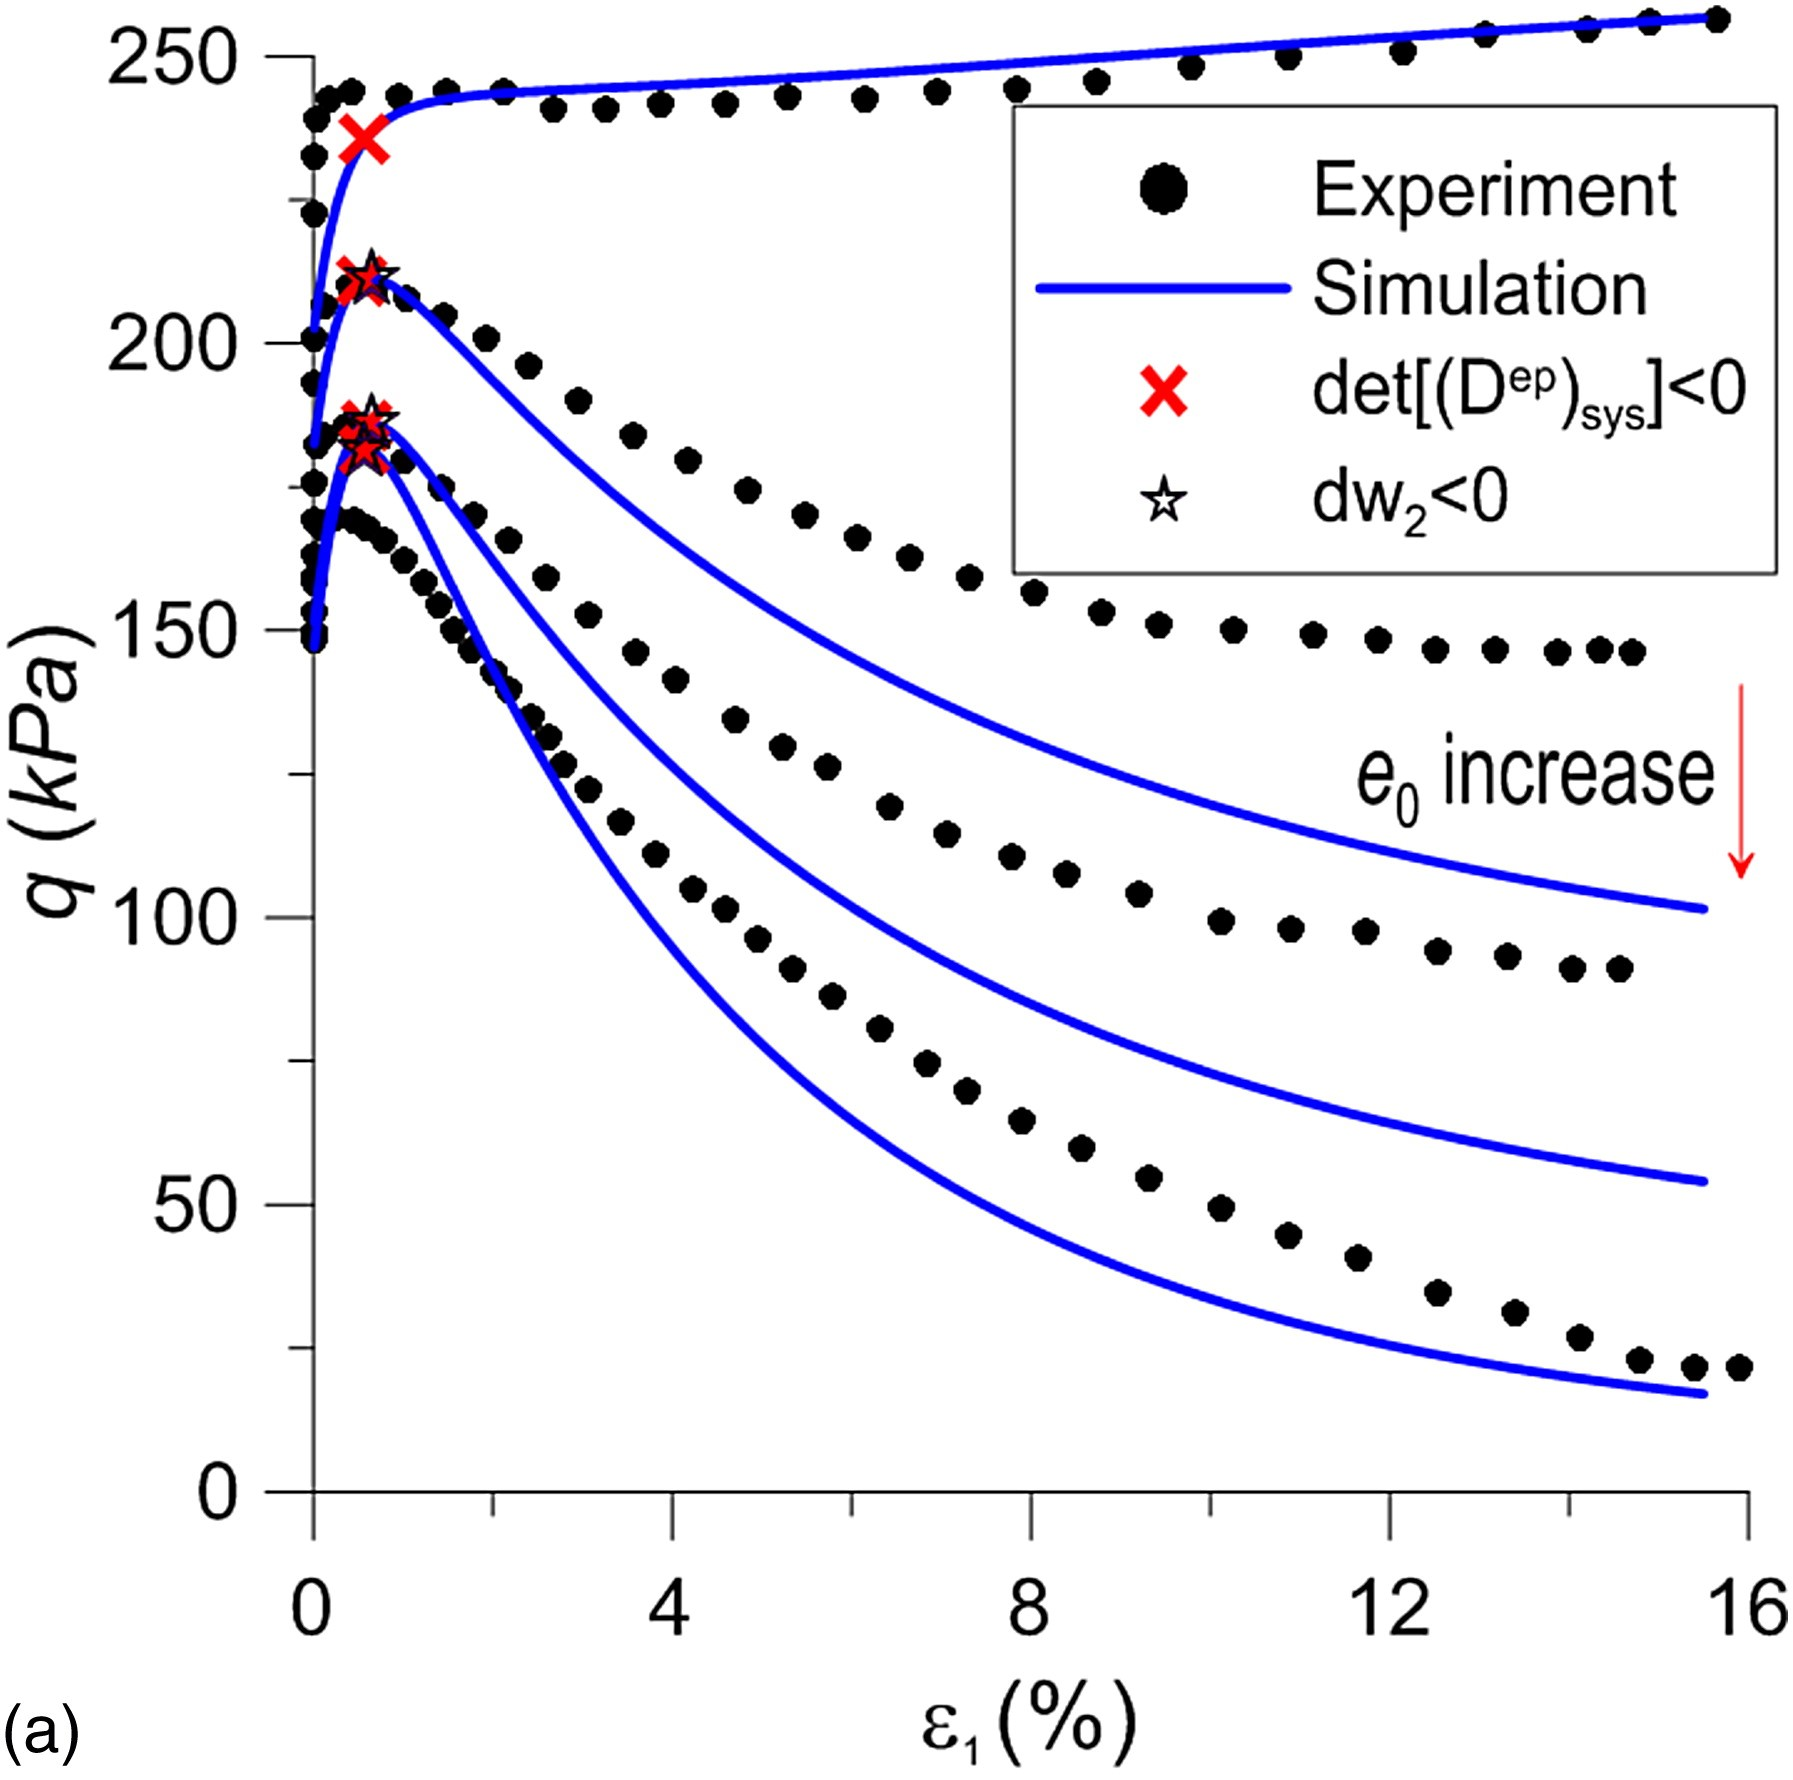
\includegraphics[width=.8\textwidth]{figures/figure10a.jpg}
                \label{figure:10a}
            }
            \subfigure[evolution of pore-water pressure 孔隙水压力的演变]{
                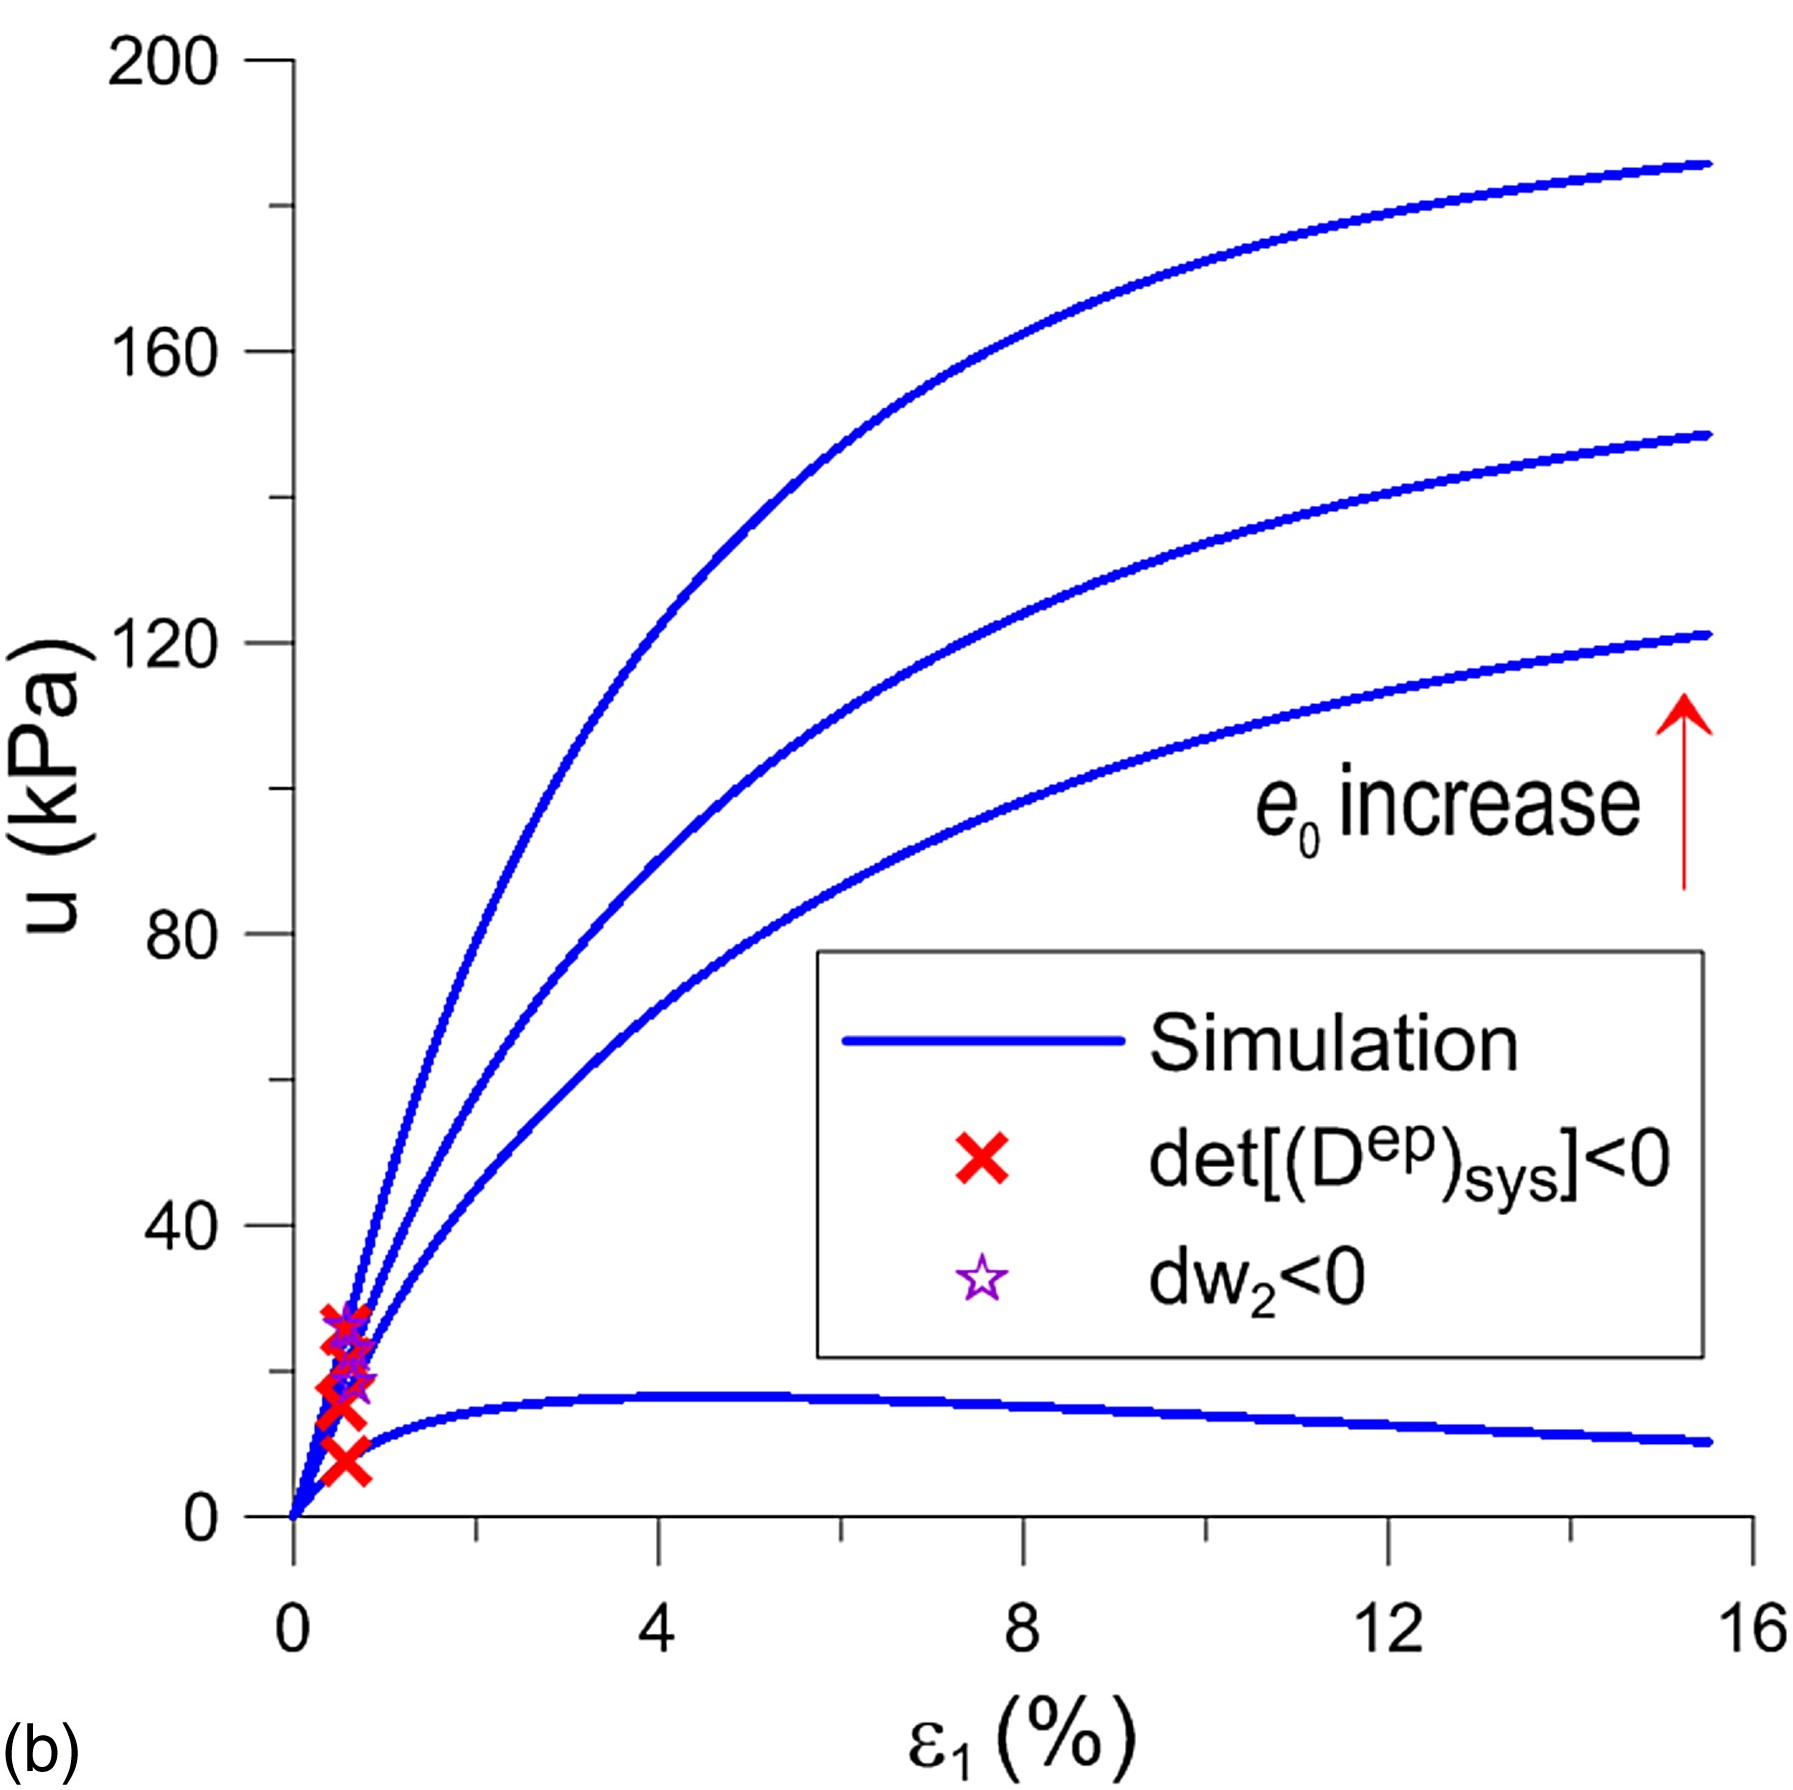
\includegraphics[width=.8\textwidth]{figures/figure10b.jpg}
                \label{figure:10b}
            }
            \bicaption{Model prediction (experimental data after Chu and \citealt{Chu2008})}{模型预测(来自\citealt{Chu2008}之后的实验数据)}
            \label{figure:10}
        \end{figure}
    \end{minipage}
\end{figure}